\documentclass[a4paper]{article}

\usepackage[T1]{fontenc}
\usepackage[utf8]{inputenc}

\usepackage{mathptmx}

\usepackage[a4paper, total={6in, 8in}]{geometry}
\usepackage{subcaption}
\usepackage[shortlabels]{enumitem}
\usepackage{amsmath,amssymb}
\usepackage{amsthm}
\usepackage{bbm}
\usepackage{graphicx}
\usepackage{float}
\usepackage[colorlinks=true,naturalnames=true,plainpages=false,pdfpagelabels=true]{hyperref}
\usepackage[parfill]{parskip}
\usepackage[backend=biber, sorting=none]{biblatex}
\addbibresource{uni.bib}
\pagestyle{myheadings}
\markright{Popovic, Vogel\hfill Unbiased Fitting \hfill}

\title{Theoretical Physics Lab-Course 2021S\\ University of Vienna \vspace{1.5cm}\\ Unbiased Fitting}
\author{Milutin Popovic \\ Tim Vogel \vspace{1.5cm}\\ Supervisor: Peter Stoffer}
\date{April 18, 2021}

\begin{document}

\maketitle

\newpage

\thispagestyle{empty}
\tableofcontents

\newpage

\section{Abstract}
\section{Introduction and Motivation}
In physics, we often come across the situation, where measured data needs to be approximated by a theoretical model,
which requires a set amount of parameters. To determine these parameters a so called "data fit" is required, which can
be done via different techniques. One of the most widely used fit-thecnique is "Least-squares fitting", but as soon
as we deal with correlated  data points, which means, each data point is not a completely independent measurement, a
wrong application of the Least-squares fit, can lead to a bias, which, in return, will affect the accuracy of the
fit in a negative way. This so called D'Agostini bias, albeit a very situational phenomenon, has to be considered when
dealing with correlated data from one or even more experiments. It can be avoided by implementing a iterative fit method and
we will consider this in an example from particle physics.
\subsection{Motivation}

\section{Physical description and Findings} %wird aus mehreren Teilen bestehen, nur als Platzhalter%
\subsection{The Vector Form Factor of Pions}
In particle physics, one of the best to study reactions of elementary particles, is
the collision between an electron $(e^-)$ and it's anti-particle, the positron ($e^+)$. When these
two particle collide, they annihilate each other and produce new types of particles. In
these experiments very precise measurements can be taken and as such, be a very valuable base
of empirical data of the Standard model of physics. A central point of study, of these
electron-positron-collisions has been the anomalous magnetic moment g-2 of the muon.
The anomaly of this number comes from the fact, that the measured data differs to the
theoretical model by quite a large margin. As such it could be the source of exciting discoveries.
The theoretical value of the g-2 momentum relies on data from the aforementioned collisions,
which is used to reconstruct the so called hadronic vacuum polarization. The hadronic vacuum
polarization itself comes from the hadronic final states. About 70\% of the contribution to
the g-2 momentum comes from the annihilation of an electron and a positron into two pions.
The probability of this happening is dependent on the energy of the two particles.
The strong interaction between these two pions is given by the so called pion vector
form factor (VFF, $F_\pi^V$).
\subsection{The D'Agostini bias}
The D'Agostini bias was first introduced by Giuilo D'Agostini in 1994. It describes a problem
with data-fits, when considering data with overall systematic errors, that share a uncertainty
on the normalization factor. In such a situation, if the error matrix $V$ of the data points is
known, one would normally minimize the $\chi^2$, which can be obtained by
$\chi^2=\vec{\Lambda}^T\cdot V^{-1}\cdot\vec{\Lambda}$. In this formula, $\Lambda$ denotes the vector
between the values of the theoretical model and the measured ones. But, after carrying out such a fit, one
often obtains results, which contradict expectations. For example, if we got the results $8.0\pm 2\%$
and $8.5\pm 2\%$, from a measurement, which share a $10\%$ normalization error, if
we minimized the $\chi^2$ as described-with the matrix $V$ estimated by the data, we would obtain the value
$7.87\pm 0.81$. This result should immediately take attention, as the result with the
highest probability, lies outside the range of the measured values. This error also occurs in
a situation, where data is taken from two or more independently conducted experiments, which are afflicted
by an additional systematic normalization error, even though the dimensions of the error are
not quite as severe as in the situation described before.
\subsection{Iterative solution to the D'Agostini bias}

\subsection{Code Structure}
Here the logical structure of the code is shown.
\begin{itemize}
    \item Construct statistical covariance matrix
    \item Construct Jacobi matrix of model function in terms of the parameters
    \item Guess initial parameters $\vec{p_0}$
    \item Iterate
        \begin{itemize}
            \item[-] Construct System covariance matrix with $\vec{p_{i}}$
            \item[-] Fill Jacobi matrix with $\vec{p_{i}}$ which is the Design Matrix
            \item[-] Claculate step $\delta \vec{p_{i}}$
            \item[-] update initial parameters
                \begin{align*}
                    \vec{p_{i+1}} = \vec{p_{i}} + \alpha \cdot \delta \vec{p_{i}} \;\;\;\;\; \alpha = 0.1
                \end{align*}
        \end{itemize}
    \item Calculate errors
    \item Calculate $\chi^2_{min}$
\end{itemize}

The guess used for all fits was determined by standard least-square fit
provided by \texttt{scipy}.
    \begin{align}
            \vec{p_0} =
            \begin{pmatrix}
            900,\; 200,\; 810,\; 40,\; 20,\; -1000,\; 840,\; 1550
            \end{pmatrix}
    \end{align}

The code can be viewed and/or downloaded from here \cite{code}
(including the calculation of the guess parameters).


\section{Results}
In this section the results with consideration of the D'Agostini are shown.
Furthermore the findings with fits of two experiments together
(6 combinations of two) and also a fit with all experiments
are shown. In the end of the section the fitted parameters are compared with
the literature values. The plots of the given data and fitted models can be found in Section \ref{plots}.

\newpage
\subsection{Single Experiment Fits under consideration of the D'Agostini bias}
In this section the data is fitted under consideration of the D'Agostini bias of all experiments separately.
\begin{table}[h!]
    \caption{Results of all experiment data fitted separately\label{tabs}}
    \centering
    \begin{tabular}{|c|c|c|c|c|}
        \hline
        $\vec{p}$ & SND & CMD2 & KLOE & BABAR \\ \hline
        $M_{\rho}$    [MeV]          & $772.72	\pm 0.59$ & $773.93	\pm 0.67$ &$773.91	\pm 0.25 $&$773.33	\pm 0.43$ \\
        $\Gamma_{\rho}$   [MeV]      & $149.53	\pm 1.15$ & $147.67	\pm 1.32$ &$149.72	\pm 0.37 $&$149.19	\pm 0.81$\\
        $M_{\omega}$      [MeV]      & $781.94	\pm 0.09$ & $782.32	\pm 0.07$ &$782.44	\pm 0.11 $&$782.18	\pm 0.07$\\
        $\Gamma_{\omega}$    [MeV]   & $8.55	\pm 0.33    $ & $8.65	\pm 0.44$ &$9.66	\pm 0.33 $&$8.17	\pm 0.16$\\
        $\varepsilon_{\omega}$ [] & $2.02	\pm 0.09    $ & $1.92	\pm 0.12$ &$2.07	\pm 0.05 $&$1.95	\pm 0.03$\\
        \hline \hline
        $\chi^2_{min}/dof$      & $1.001$&$ 1.054$&$ 1.443$&$ 1.031$\\
        $p\text{-value}$        & $0.530$&$ 0.395$&$ 0.001$&$ 0.377$\\
        \hline
    \end{tabular}
\end{table}

\subsection{Multi Experiment Fits under consideration of the D'Agostini bias}
In this section the data is fitted considering the D'Agostini bias, first the data of
two experiments together then the data of all experiments.

\begin{table}[h!]
    \caption{Results of data fits of experimental data fitted in pairs}
    \centering
    \begin{tabular}{|c|c|c|c|}
        \hline
        $\vec{p}$ & SND-CMD2 & SND-KLOE & SND-BABAR  \\ \hline
        $M_{\rho}$[MeV]              & $772.72	\pm 0.42$ & $773.92	\pm 0.23$ &$773.17	\pm 0.36 $ \\
        $\Gamma_{\rho}$[MeV]         & $149.53	\pm 0.81$ & $149.42	\pm 0.35$ &$149.70	\pm 0.64 $\\
        $M_{\omega}$  [MeV]          & $781.95	\pm 0.07$ & $782.39	\pm 0.07$ &$782.07	\pm 0.06 $\\
        $\Gamma_{\omega}$ [MeV]      & $8.56	\pm 0.24    $ & $9.42	\pm 0.20$ &$8.27	\pm 0.13 $\\
        $\varepsilon_{\omega}$[]  & $2.02	\pm 0.07    $ & $2.07	\pm 0.05$ &$1.96	\pm 0.03 $\\
        \hline \hline
        $\chi^2_{min}/dof$      & $0.904$&$ 1.839$&$ 0.945$\\
        $p\text{-value}$        & $0.754$&$ 0.001$&$ 0.763$\\
        \hline

    \end{tabular}
\end{table}


\begin{table}[h!]
    \caption{Results of data fits of experimental data fitted in pairs}
    \centering
    \begin{tabular}{|c|c|c|c|}
        \hline
        $\vec{p}$ & CMD2-KLOE & CMD2-BABAR & KLOE-BABAR  \\ \hline
        $M_{\rho}$        [MeV]      & $773.92	\pm 0.23$ & $773.17	\pm 0.36$ &$773.66	\pm 0.20 $ \\
        $\Gamma_{\rho}$     [MeV]    & $149.42	\pm 0.35$ & $149.70	\pm 0.64$ &$149.41	\pm 0.32 $\\
        $M_{\omega}$         [MeV]   & $782.39	\pm 0.07$ & $782.07	\pm 0.06$ &$782.49	\pm 0.06 $\\
        $\Gamma_{\omega}$    [MeV]   & $9.42	\pm 0.02    $ & $8.27	\pm 0.13$ &$8.98	\pm 0.12 $\\
        $\varepsilon_{\omega}$ [] & $2.07	\pm 0.05    $ & $1.96	\pm 0.03$ &$1.98	\pm 0.02 $\\
        \hline \hline
        $\chi^2_{min}/dof$      & $1.838$&$ 0.943$&$ 1.470$\\
        $p\text{-value}$        & $0.001$&$ 0.772$&$ 0.001$\\
        \hline

    \end{tabular}
\end{table}

\begin{table}[h!]
    \caption{Results of data fit of all experimental data fitted together\label{tabmulti}}
    \centering
    \begin{tabular}{|c|c|}
        \hline
        $\vec{p}$   & Multi-Fit\\
        \hline
        $M_{\rho}$       [MeV]       & $773.62	\pm 0.18$   \\
        $\Gamma_{\rho}$     [MeV]    & $149.42	\pm 0.29$  \\
        $M_{\omega}$         [MeV]   & $782.36	\pm 0.08$  \\
        $\Gamma_{\omega}$   [MeV]    & $8.75	\pm 0.08    $  \\
        $\varepsilon_{\omega}$[]  & $1.96	\pm 0.02    $  \\
        \hline \hline
        $\chi^2_{min}/dof$      & $1.735$\\
        $p\text{-value}$        & $0.000$\\
        \hline

    \end{tabular}
\end{table}

\subsection{Litrature comparison}
In this section the fitted parameters of CMD2-BABAR and the literature values\cite{particleref} are compared.
The reason why CMD2-BABAR was chosen, is that it has a value of $\chi^2_{min}$ close to $1$.
\begin{table}[ht!]
    \caption{Result comparison with literature\label{tabref}}
    \centering
    \begin{tabular}{|l|c|c|c|}
        \hline
        $\vec{p}$     & Literature    &   CMD2-BABAR      & Relative error \\
        \hline
        $M_{\rho}$   [MeV]           & $775.26	\pm 0.25$ & $773.17	\pm 0.36$ & $ 0.02 \%$\\
        $\Gamma_{\rho}$   [MeV]      & $147.80	\pm 0.90$  & $149.70	\pm 0.64$  & $ 1.02 \%$ \\
        $M_{\omega}$       [MeV]     & $782.65	\pm 0.12$  & $782.07	\pm 0.06$ & $ 0.0008\% $ \\
        $\Gamma_{\omega}$  [MeV]     & $8.49	\pm 0.08    $ & $8.27	\pm 0.13$  & $ 0.03 \%$\\
        \hline
    \end{tabular}
\end{table}

\subsection{Fitting with D'Agostini bias}
Furthermore here we compare the results of the t0-method, with the incorrect method of
multiplying the relative systematic uncertainties with the data provided, instead of
calculating the systematic uncertainties in regards of the newly calculated parameters in
every iteration. For demonstrational purposes only the single fitted experiments are pulled.
Again we would like to reference the plots in Section \ref{plots}. In the following table
the results of the incorrect method applied to fitting are shown.

\begin{table}[h!]
    \caption{Results of all experiment data wrongly fitted  separately}
    \centering
    \begin{tabular}{|c|c|c|c|c|}
        \hline
        $\vec{p}$ & SND & CMD2 & KLOE & BABAR \\ \hline
        $M_{\rho}$   [MeV]           & $772.21	\pm 4.97$ & $774.51	\pm 2.59$ &$774.09	\pm 0.25 $&$773.42 \pm 0.54$ \\
        $\Gamma_{\rho}$   [MeV]      & $151.26	\pm 13.11$ & $145.18	\pm 5.83$ &$149.89	\pm 0.84 $&$149.29	\pm 1.01$\\
        $M_{\omega}$      [MeV]      & $781.03	\pm 0.47$ & $782.09	\pm 0.32$ &$782.79	\pm 0.18 $&$782.18	\pm 0.07$\\
        $\Gamma_{\omega}$  [MeV]     & $8.96	\pm 2.25    $ & $8.58	\pm 0.15$ &$11.11	\pm 0.70 $&$8.18	\pm 0.18$\\
        $\varepsilon_{\omega}$[]  & $2.14	\pm 0.68    $ & $1.85	\pm 0.38$ &$2.15	\pm 0.08 $&$1.94	\pm 0.04$\\
        \hline \hline
        $\chi^2_{min}/dof$      & $0.016$&$ 0.125$&$ 0.903$&$ 1.118$\\
        $p\text{-value}$        & $1.000$&$ 1.000$&$ 0.839$&$ 0.099$\\
        \hline
    \end{tabular}
\end{table}

Obviously the results are much worse than in Table \ref{tabs}.

\subsubsection{Plots\label{plots}}
\begin{figure}[H]
    \centering
    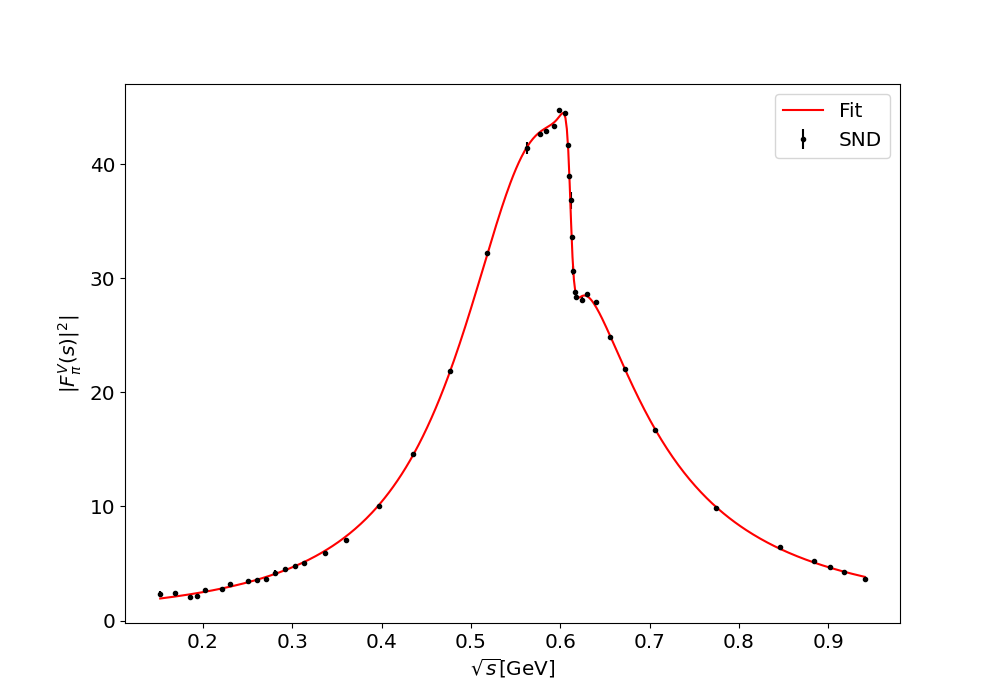
\includegraphics[width=0.8\textwidth]{./plots/SND.png}
    \caption{SND data fit\label{fig1}}
\end{figure}
\begin{figure}[H]
    \centering
    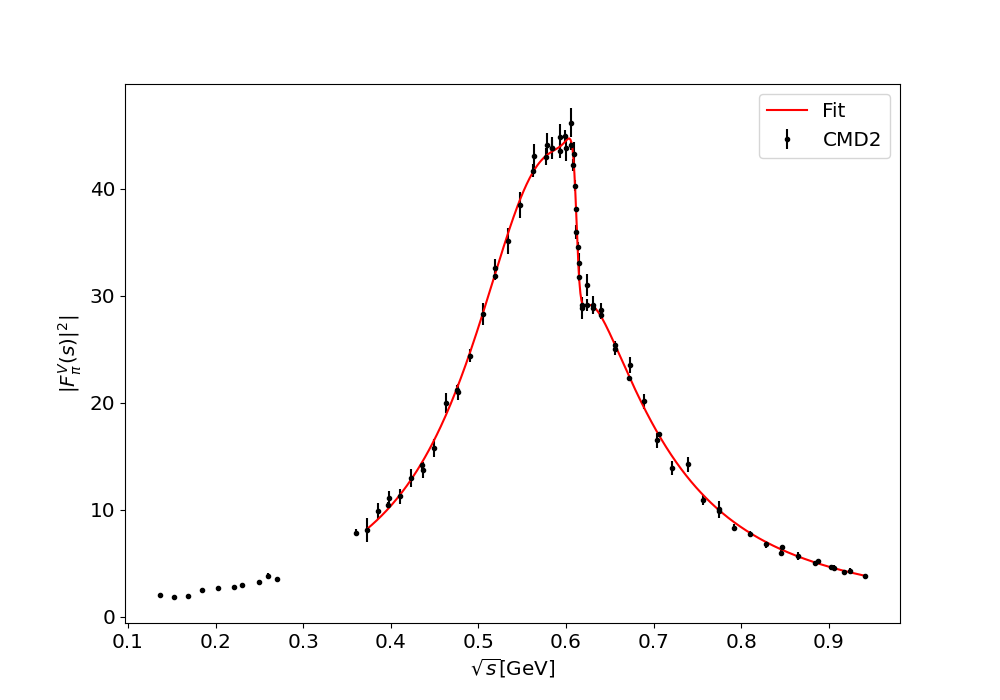
\includegraphics[width=0.8\textwidth]{./plots/CMD2.png}
    \caption{CMD2 data fit\label{fig2}}
\end{figure}
\begin{figure}[H]
    \centering
    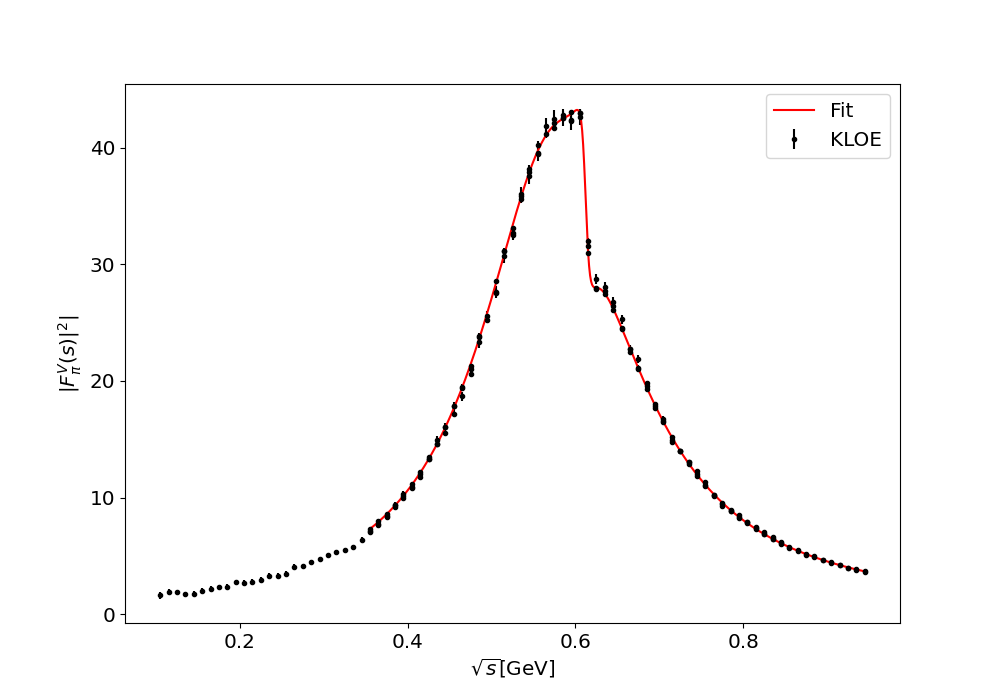
\includegraphics[width=0.8\textwidth]{./plots/KLOE.png}
    \caption{KLOE data fit\label{fig3}}
\end{figure}
\begin{figure}[H]
    \centering
    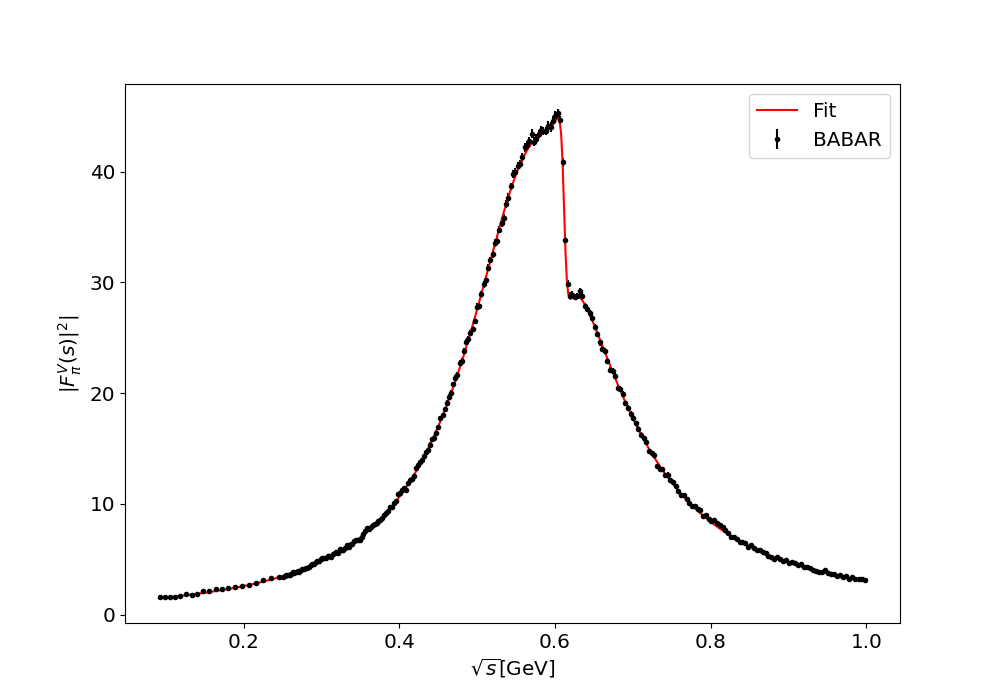
\includegraphics[width=0.8\textwidth]{./plots/BABAR.png}
    \caption{BABAR data fit\label{fig4}}
\end{figure}



\begin{figure}[H]
    \centering
    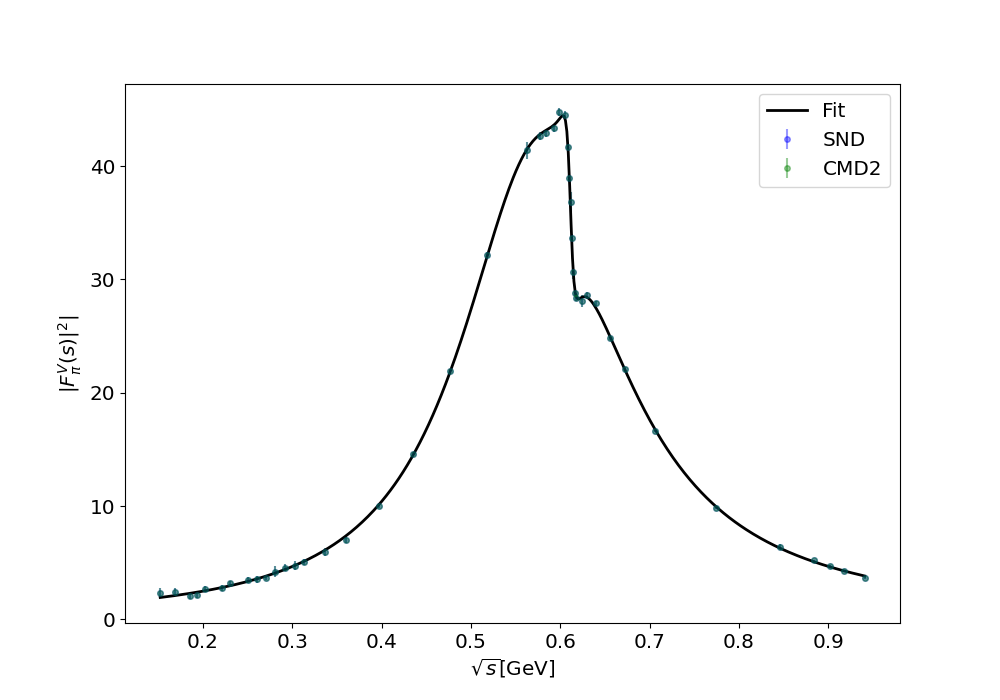
\includegraphics[width=0.8\textwidth]{./plots/SND-CMD2.png}
    \caption{SND and CMD2 fitted togther\label{fig5}}
\end{figure}
\begin{figure}[H]
    \centering
    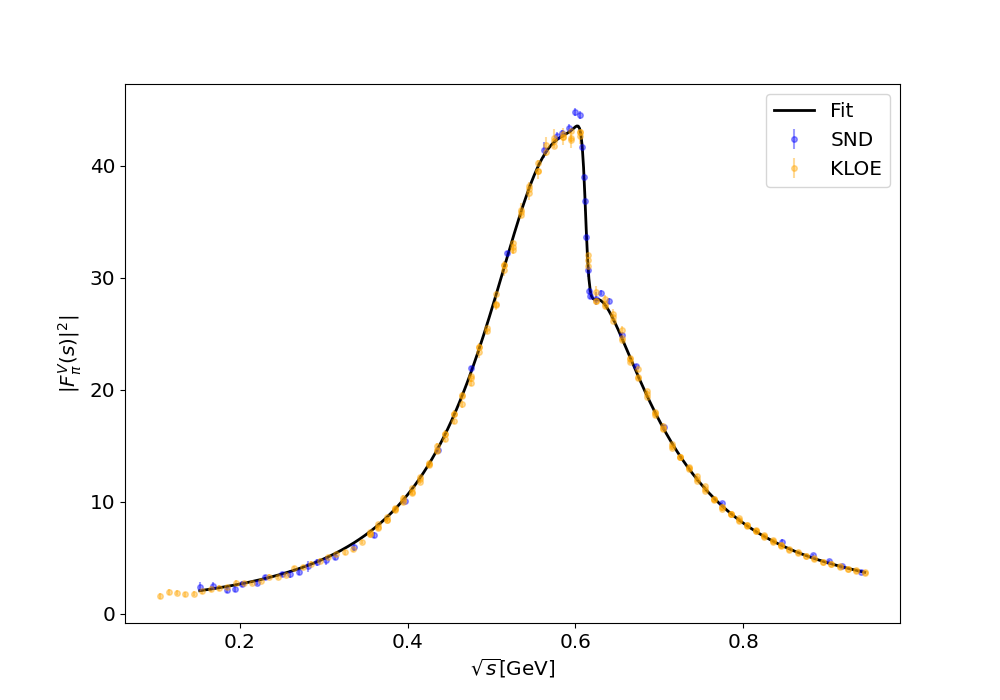
\includegraphics[width=0.8\textwidth]{./plots/SND-KLOE.png}
    \caption{SND and KLOE fitted togther    \label{fig6}}
\end{figure}
\begin{figure}[H]
    \centering
    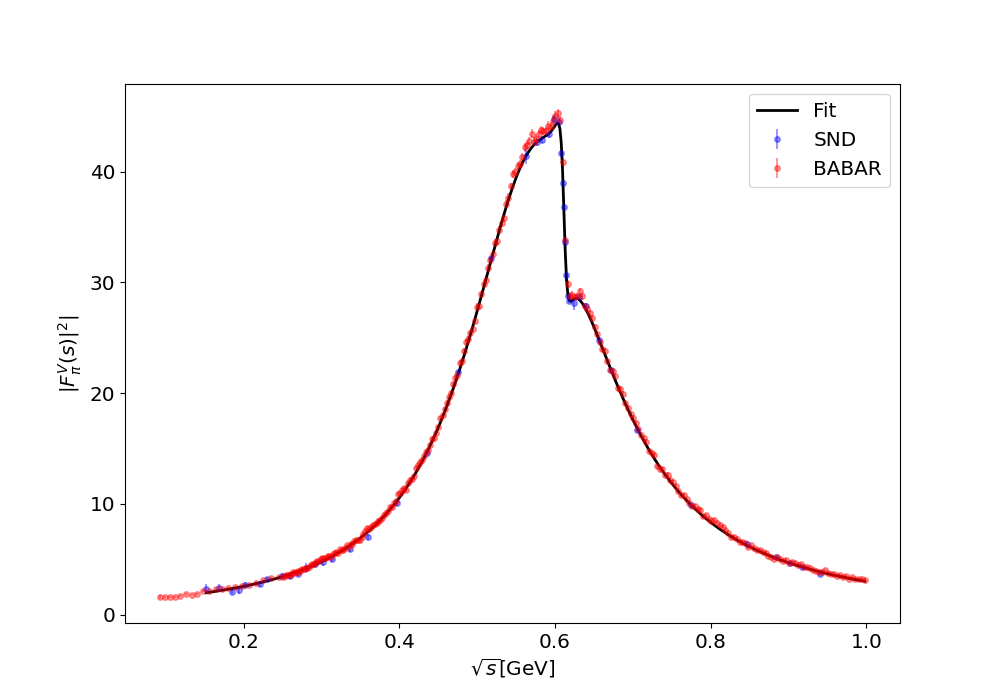
\includegraphics[width=0.8\textwidth]{./plots/SND-BABAR.png}
    \caption{SND and BABAR fitted togther   \label{fig7}}
\end{figure}


\begin{figure}[H]
    \centering
    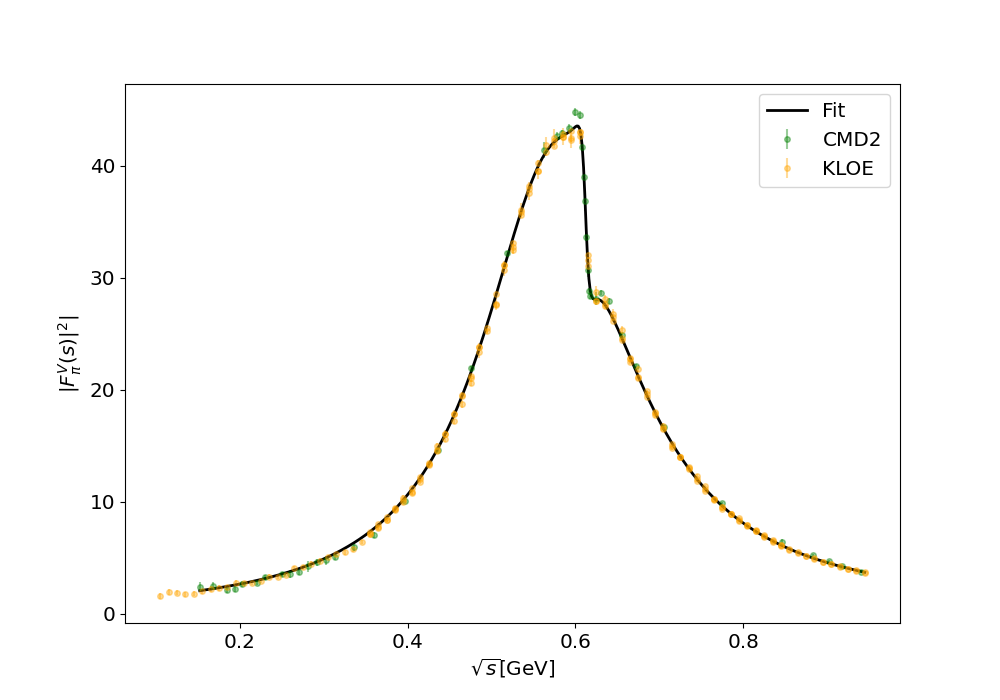
\includegraphics[width=0.8\textwidth]{./plots/CMD2-KLOE.png}
    \caption{CMD2 and KLOE fitted togther   \label{fig8}}
\end{figure}
\begin{figure}[H]
    \centering
    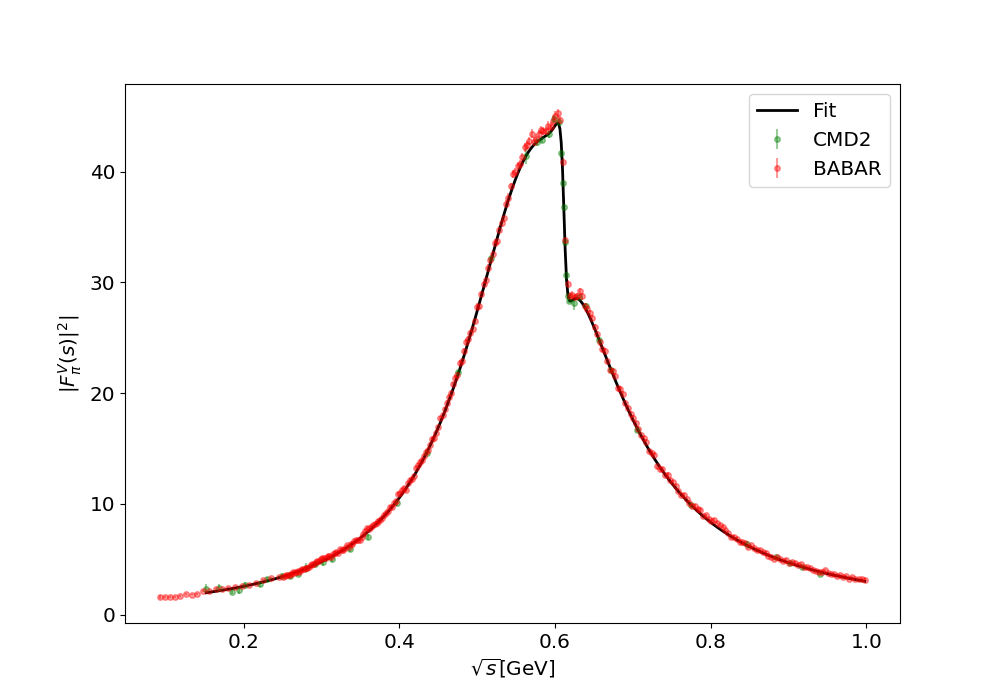
\includegraphics[width=0.8\textwidth]{./plots/CMD2-BABAR.png}
    \caption{CMD2 and BABAR fitted togther   \label{fig9}}
\end{figure}
\begin{figure}[H]
    \centering
    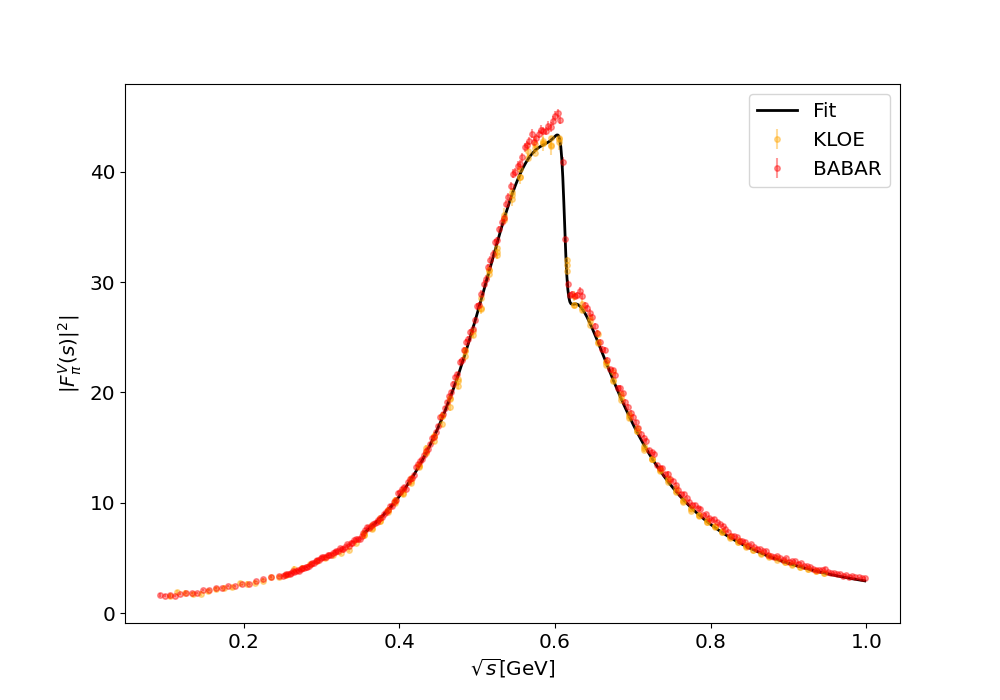
\includegraphics[width=0.8\textwidth]{./plots/KLOE-BABAR.png}
    \caption{KLOE and BABAR fitted togther   \label{fig10}}
\end{figure}

\begin{figure}[H]
    \centering
    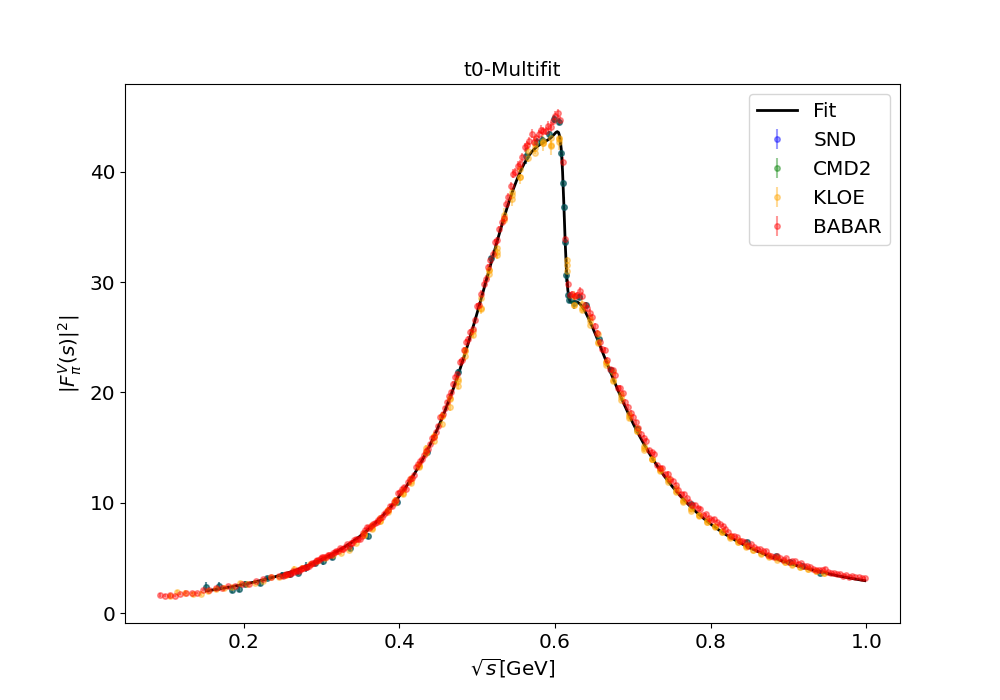
\includegraphics[width=0.8\textwidth]{./plots/multi.png}
    \caption{SND, CMD, KLOE and BABAR fitted togther   \label{fig10}}
\end{figure}

\begin{figure}[H]
    \centering
    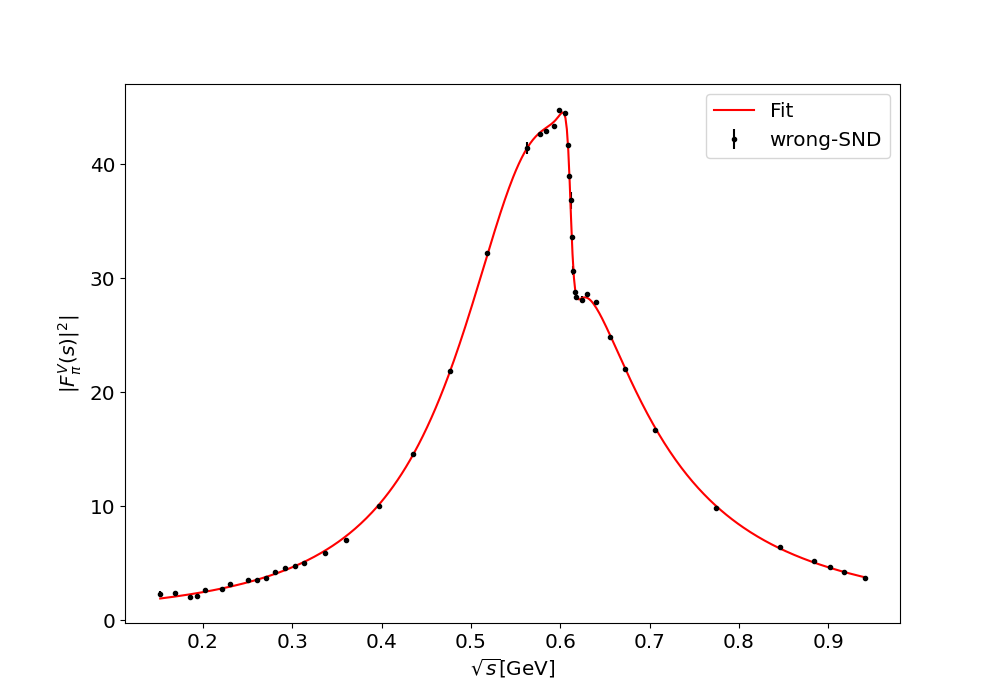
\includegraphics[width=0.8\textwidth]{./plots/wrong-SND.png}
    \caption{Wrong method, SND data fit\label{fig1}}
\end{figure}
\begin{figure}[H]
    \centering
    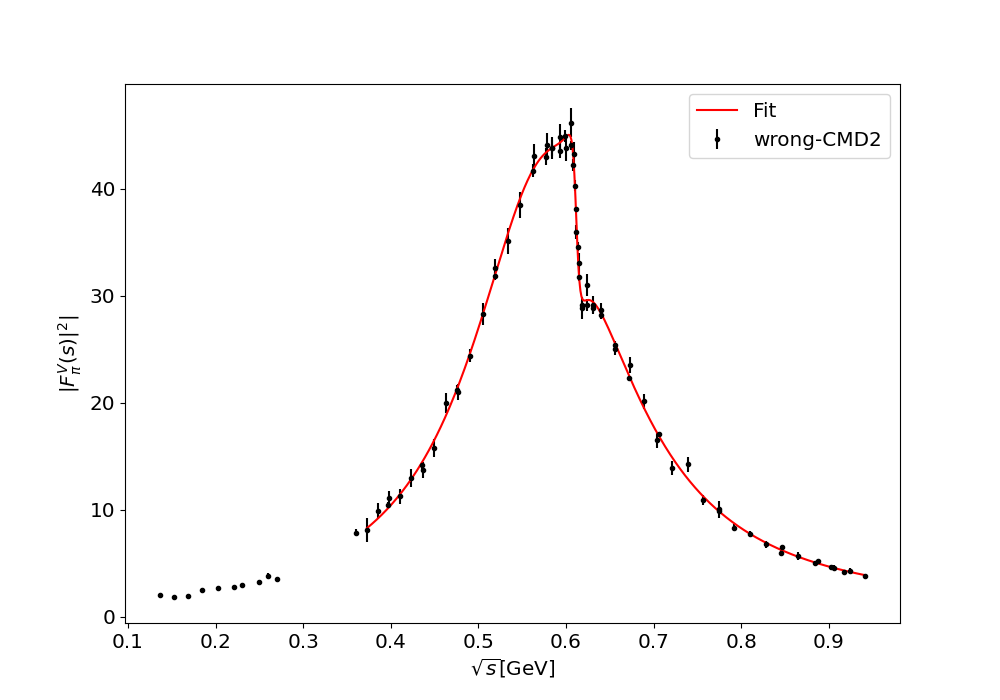
\includegraphics[width=0.8\textwidth]{./plots/wrong-CMD2.png}
    \caption{Wrong method, CMD2 data fit\label{fig2}}
\end{figure}
\begin{figure}[H]
    \centering
    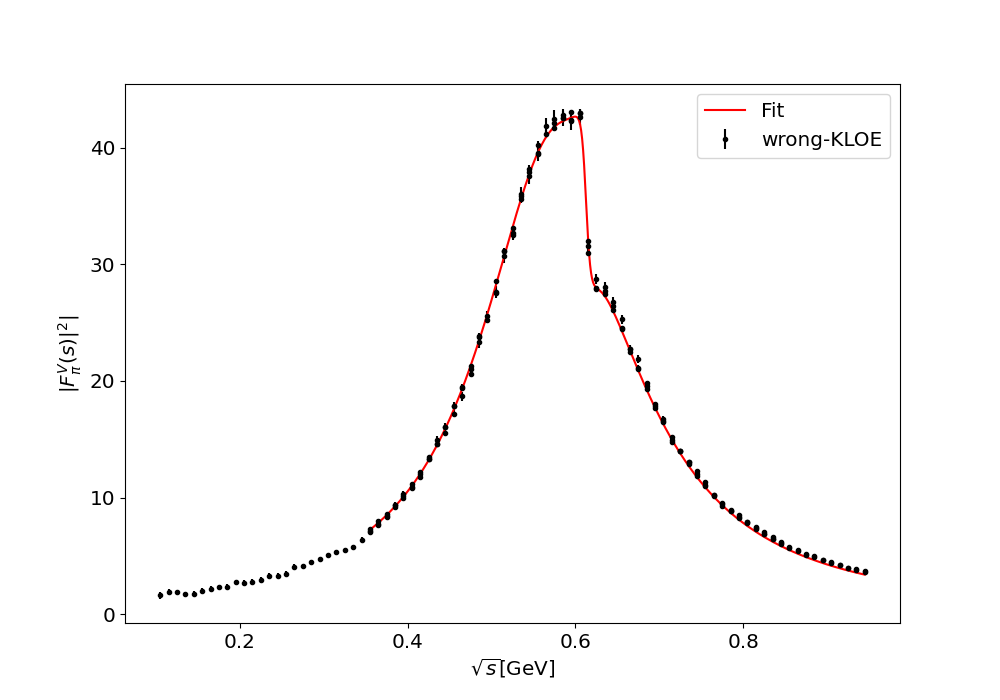
\includegraphics[width=0.8\textwidth]{./plots/wrong-KLOE.png}
    \caption{Wrong method, KLOE data fit\label{fig3}}
\end{figure}
\begin{figure}[H]
    \centering
    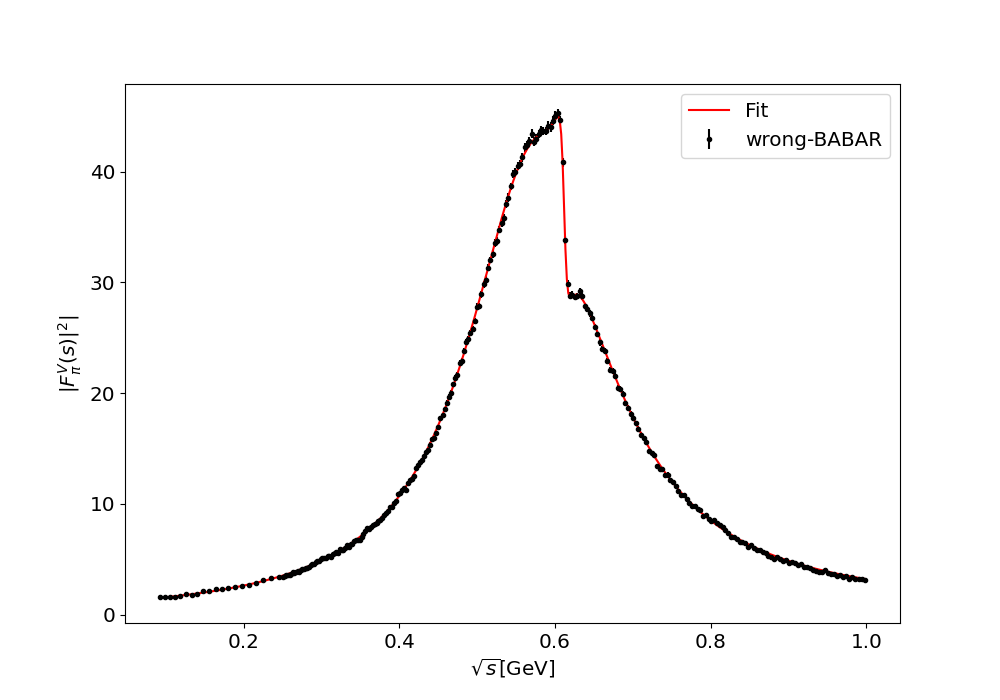
\includegraphics[width=0.8\textwidth]{./plots/wrong-BABAR.png}
    \caption{Wrong method, BABAR data fit\label{fig4}}
\end{figure}

\printbibliography

\end{document}
